\documentclass[]{book}
\usepackage{lmodern}
\usepackage{amssymb,amsmath}
\usepackage{ifxetex,ifluatex}
\usepackage{fixltx2e} % provides \textsubscript
\ifnum 0\ifxetex 1\fi\ifluatex 1\fi=0 % if pdftex
  \usepackage[T1]{fontenc}
  \usepackage[utf8]{inputenc}
\else % if luatex or xelatex
  \ifxetex
    \usepackage{mathspec}
  \else
    \usepackage{fontspec}
  \fi
  \defaultfontfeatures{Ligatures=TeX,Scale=MatchLowercase}
\fi
% use upquote if available, for straight quotes in verbatim environments
\IfFileExists{upquote.sty}{\usepackage{upquote}}{}
% use microtype if available
\IfFileExists{microtype.sty}{%
\usepackage{microtype}
\UseMicrotypeSet[protrusion]{basicmath} % disable protrusion for tt fonts
}{}
\usepackage{hyperref}
\hypersetup{unicode=true,
            pdftitle={User Guide for the MUX},
            pdfauthor={MultiplexÔ},
            pdfborder={0 0 0},
            breaklinks=true}
\urlstyle{same}  % don't use monospace font for urls
\usepackage{natbib}
\bibliographystyle{apalike}
\usepackage{longtable,booktabs}
\usepackage{graphicx,grffile}
\makeatletter
\def\maxwidth{\ifdim\Gin@nat@width>\linewidth\linewidth\else\Gin@nat@width\fi}
\def\maxheight{\ifdim\Gin@nat@height>\textheight\textheight\else\Gin@nat@height\fi}
\makeatother
% Scale images if necessary, so that they will not overflow the page
% margins by default, and it is still possible to overwrite the defaults
% using explicit options in \includegraphics[width, height, ...]{}
\setkeys{Gin}{width=\maxwidth,height=\maxheight,keepaspectratio}
\IfFileExists{parskip.sty}{%
\usepackage{parskip}
}{% else
\setlength{\parindent}{0pt}
\setlength{\parskip}{6pt plus 2pt minus 1pt}
}
\setlength{\emergencystretch}{3em}  % prevent overfull lines
\providecommand{\tightlist}{%
  \setlength{\itemsep}{0pt}\setlength{\parskip}{0pt}}
\setcounter{secnumdepth}{5}
% Redefines (sub)paragraphs to behave more like sections
\ifx\paragraph\undefined\else
\let\oldparagraph\paragraph
\renewcommand{\paragraph}[1]{\oldparagraph{#1}\mbox{}}
\fi
\ifx\subparagraph\undefined\else
\let\oldsubparagraph\subparagraph
\renewcommand{\subparagraph}[1]{\oldsubparagraph{#1}\mbox{}}
\fi

%%% Use protect on footnotes to avoid problems with footnotes in titles
\let\rmarkdownfootnote\footnote%
\def\footnote{\protect\rmarkdownfootnote}

%%% Change title format to be more compact
\usepackage{titling}

% Create subtitle command for use in maketitle
\providecommand{\subtitle}[1]{
  \posttitle{
    \begin{center}\large#1\end{center}
    }
}

\setlength{\droptitle}{-2em}

  \title{User Guide for the MUX}
    \pretitle{\vspace{\droptitle}\centering\huge}
  \posttitle{\par}
    \author{MultiplexÔ}
    \preauthor{\centering\large\emph}
  \postauthor{\par}
      \predate{\centering\large\emph}
  \postdate{\par}
    \date{2019-07-18}

\usepackage{booktabs}
\usepackage{amsthm}
\makeatletter
\def\thm@space@setup{%
  \thm@preskip=8pt plus 2pt minus 4pt
  \thm@postskip=\thm@preskip
}
\makeatother

\begin{document}
\maketitle

{
\setcounter{tocdepth}{1}
\tableofcontents
}
\hypertarget{reasons-for-the-mux}{%
\chapter{Reasons for the MUX}\label{reasons-for-the-mux}}

The first prototype of the system was built in 2010. The idea was that current water quality sensors are expensive and they are designed to be installed to obtain high frequency data at a particular station. In the field of hydrology, agrohydrology, ecohydrology, and limnology, to only name a few, there is a tight coupling between concentration variations in time and those in space. In other words, concentrations may vary by several folds within minutes and meters. To be able to track constituents and their fate over short distances (\textasciitilde{}\textless{} 50 m), one would ideally need not \emph{\textbf{one}} but \emph{\textbf{several}} sensors\ldots{} But then the price of such monitoring system would be prohibitive in the vast majority of cases. Not to mention that maintenance and chances of failure would be multiplied by the number of sensors deployed.

A more promising idea was to create a system that would be able to provide access to high enough frequency data for \emph{\textbf{multiple points}} in the vicinity of \emph{\textbf{one sensor}}. This solves the affordability problem as one sensor only is necessary, and it also solves the problem of multiplying maintenance on multiple sensors. Our solution is the MultiPlexed, MultiPoint Sampler or MPS, which we have now decided to call the \emph{MUX}, because it is just easier to say! And since you have the instrument with you now, you probably already have a pretty good idea of how it works.

\begin{figure}

{\centering 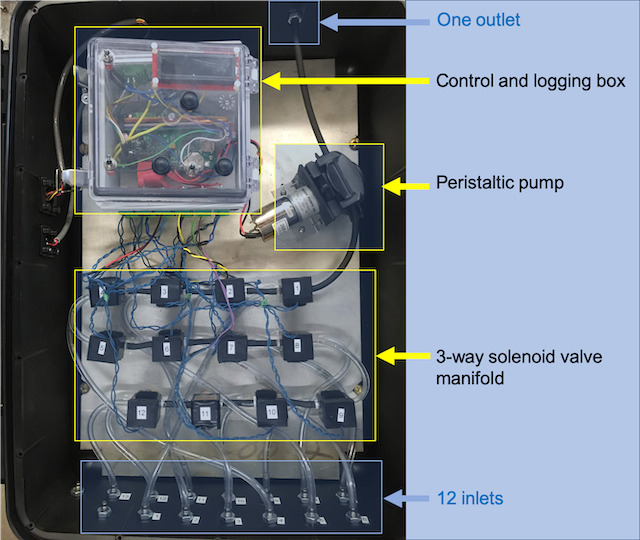
\includegraphics[width=0.8\linewidth]{pictures/MUXLayout} 

}

\caption{General Layout of the MUX, including a control box, a peristaltic pump, 12 3-way solenoid valves, 12 inlets, and one outlet}\label{fig:MUXLayout}
\end{figure}

Our solution is thus to bring water to the sensor, rather than the opposite. And once this idea became a promising solution, then expanding the `bringing of water to the sensor' to multiple points was a natural extension of the idea. All the MUX is, is a peristaltic pump for pumping and purging, a bunch of three-way solenoid valves (we chose 12 for now) that dictate which sampling point is activated, and a micro controller system to control and log all the MUX activities in synchrony with the sensor (Figure \ref{fig:MUXLayout}). The MUX sequentially pumps water from all the desired point to the sensor, and once all the points have been sampled, the sequence starts over again.

In theory, it is very simple. In practice, we have discovered that it takes a lot of attention to details to have a system that is robust enough to work over long periods of time reliably. We feel the version we have now is robust enough for others to use, although we are quite aware that there is still room for improvement, and we are dedicated to keep improving our system. We have published the details of the design and the performance of the MUX in \citeyearpar{Birgand2016-to}.

\hypertarget{the-versions-available}{%
\section{The versions available}\label{the-versions-available}}

Right now, we have three versions available. One specifically dedicated to work with the S::CAN field spectrophotometer called Spectro::lyser, one version that works with any sensor, and, a third version coupled with a synchronous syringe based sampler designed to sample rather small volumes of water at very low pumping rates (\textasciitilde{}around 1 ml/min).

\hypertarget{intro}{%
\chapter{How to hook things together}\label{intro}}

\hypertarget{the-different-parts}{%
\section{The different parts}\label{the-different-parts}}

The version you have received works with a S::CAN spectro::lyser, a Con::nect box, a power supply cable connected between a battery or a AC to DC transformer, a 12V battery (+ solar panel for long term deployment) or a AC to DC transformer, a 6-pin and a 2-pin cables provided with the MUX, and the MUX itself. You need all these parts for things to work properly.

We use only 4 of the cables of the 6-pin cable. This cable is used to catch the cleaning or valve signal from the Spectro::lyser, which we later use trigger the MUX sampling sequence, and, to obtain the measurement data through the RS485 connection and communication protocol.

We use the 2-pin cable to power the MUX. Honestly, we could have used the 6-pin cable and use all 6 cable to do, power, cleaning signal, and the data transfer, but by default, we like to keep a cable dedicated to power.

\hypertarget{connecting-with-the-connect-box}{%
\section{Connecting with the Con::nect Box}\label{connecting-with-the-connect-box}}

All wires to the MUX are connected to the Con::nect Box. To use with the MUX, we use the left panel of the Con::nect Box (Figure \ref{fig:connectboxfull}).

\begin{figure}

{\centering 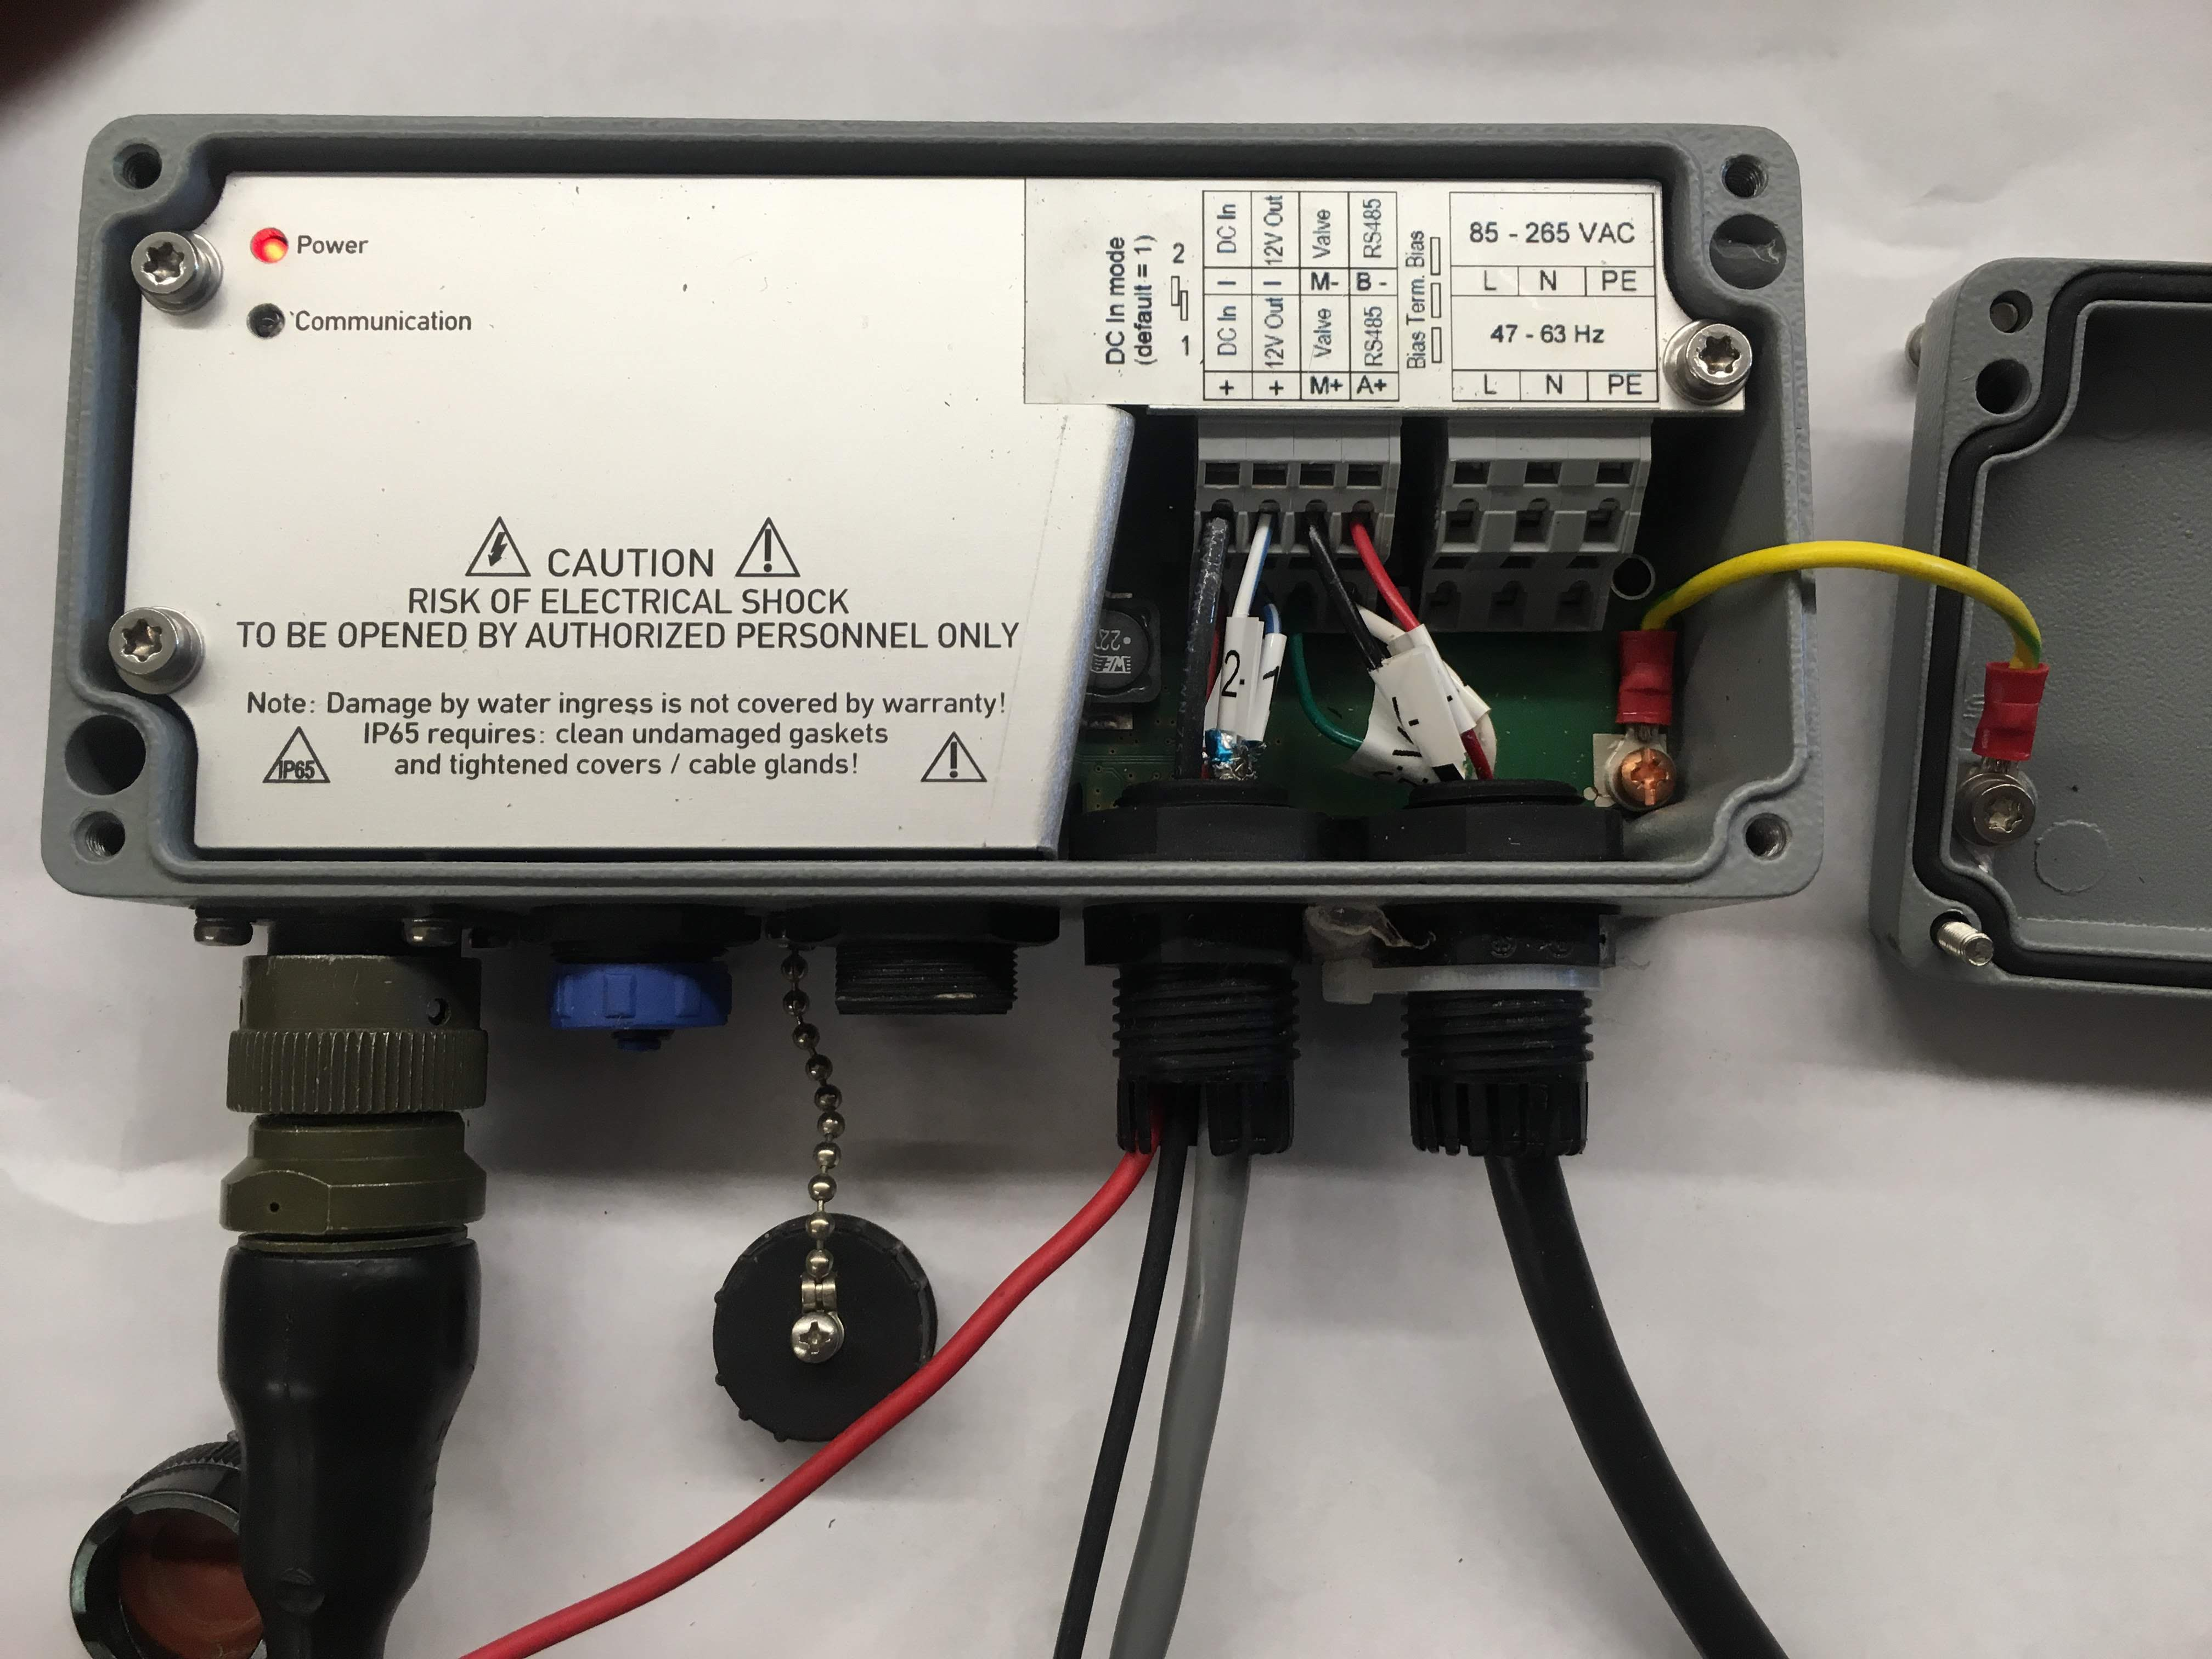
\includegraphics[width=0.7\linewidth]{pictures/ConnectBoxFull} 

}

\caption{picture of the connecting capabilities inside the Con::nect Box}\label{fig:connectboxfull}
\end{figure}

\hypertarget{powering-the-connect-box}{%
\subsection{Powering the Con::nect Box}\label{powering-the-connect-box}}

At the most left side, the user connects the wires either connected a 12V battery, or to an AC to DC adapter, which delivers 12V. This is referred to as `DC In' on the Con::nect Box label (Figure \ref{fig:connectboxfull}). By convention, the positive wire is normally red and the negative wire, black. The black or negative wire is at the top or right of the label, and the red or positive wire is at the bottom (not really visible on Figure \ref{fig:connectboxfull}). Make sure you use at least 14 gauge for these wires, to be on the safe side.

All the Con::nect Box connections are done using spring-loaded terminal. You need to use a fine screwdriver and insert it on the top part of the terminal (yellow arrows on Figure \ref{fig:SpringLoadedTerminal}), gently push or rotate down to open the spring-loaded connection located below (magenta arrows on Figure \ref{fig:SpringLoadedTerminal}). While open, insert the wire as deep as you can to obtain the best and secure connection, while still leaving the plastic sheathing out. Make sure the free wires are not longer than 4 mm, however, otherwise free wires will be stay out and that is not ideal. After you have inserted the wires, make sure you pull on the wire. If it comes out easily, do it again until it is hard to pull on it. Also, always insert the bottom wires first.

\begin{figure}

{\centering 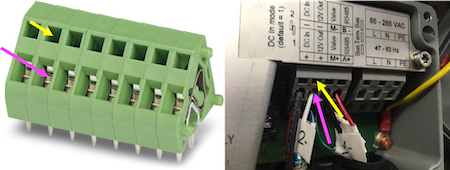
\includegraphics[width=0.9\linewidth]{pictures/SpringLoadedConnections} 

}

\caption{Spring-loaded connections for the Con::nect Box}\label{fig:SpringLoadedTerminal}
\end{figure}

The three other connection types include `12V out', `Valve', and `RS485', and we use all three with the MUX.

\hypertarget{powering-the-mux}{%
\subsection{Powering the MUX}\label{powering-the-mux}}

The MUX is powered by the `12V out' connection. The Con::nect Box provides a source of 12V power to other instruments that might be connected to it and we are taking advantage of this system to power the MUX. For that you will use the 2-pin cable as illustrated in Figure \ref{fig:2-pin-cable} below.

\begin{figure}

{\centering 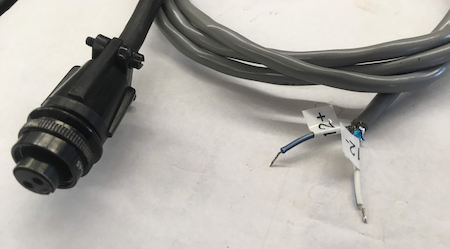
\includegraphics[width=0.7\linewidth]{pictures/2-pin-cable} 

}

\caption{2-pin cable to provide 12V DC power to the MUX, with the blue wire as '+' and the white wire as '-'}\label{fig:2-pin-cable}
\end{figure}

The blue wire corresponds to the positive or ``+'' and the white wire corresponds to the negative or `-'. As illustrated in Figure \ref{fig:ConnectBox1}, insert the blue ``+'' wire at the bottom or left connection, and the white ``-'' wire at the top or right connection of the `12V out' terminal.

\begin{figure}

{\centering 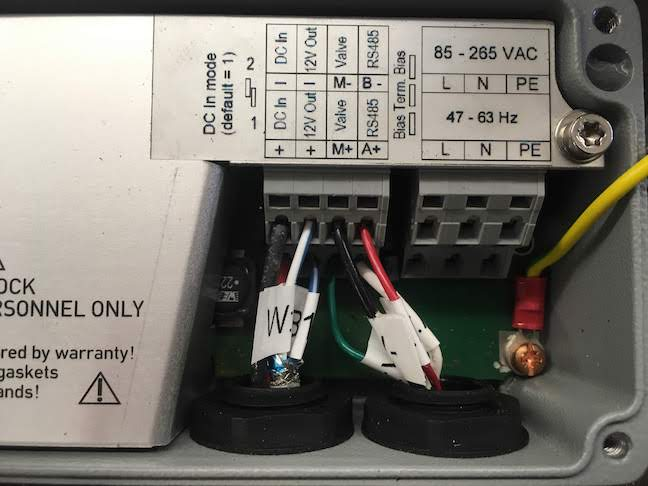
\includegraphics[width=0.7\linewidth]{pictures/ConnectBox1} 

}

\caption{2-pin cable to provide 12V DC power to the MUX, with the blue wire as '+' and the white wire as '-'}\label{fig:ConnectBox1}
\end{figure}

\hypertarget{connections-to-trigger-the-mux}{%
\subsection{Connections to Trigger the MUX}\label{connections-to-trigger-the-mux}}

The Con::nect box has a connection through which it can send a 12V signal for a specified amount of time. Actually, it is the spectro::lyser that sends the 12V. Originally, this was used to open an air valve to send a burst of compressed air to clean up the optics. Later it has been used to activate an automatic brush, also to clean the optics. We are using this feature to start a sampling sequence from the MUX. When at idle, the MUX is listening to such a 12V signal, and upon receiving this signal the MUX starts its sampling sequence.

For this we use the black and green wires of the 6-pin cable (Figure \ref{fig:6-pin-cable}).

\begin{figure}

{\centering 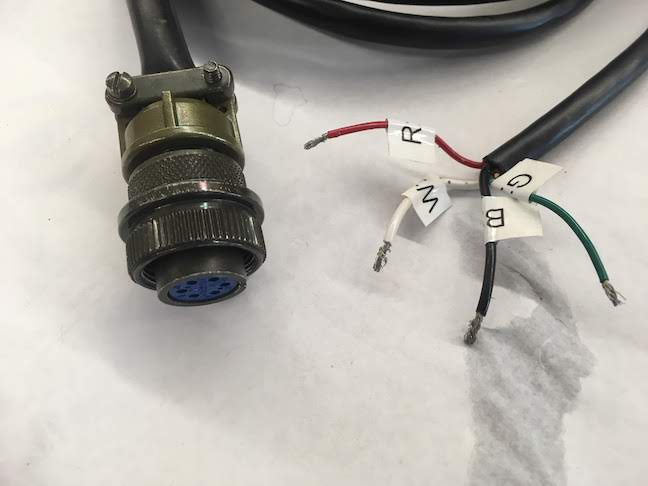
\includegraphics[width=0.8\linewidth]{pictures/6-pin-cable} 

}

\caption{6-pin cable to trigger a sampling sequence to the MUX, using the black (M-) and green (M+) wires, and, to communicate between the MUX and the spectro::lyser using the white (A+) and the red (B-) wires through the RS485 protocol}\label{fig:6-pin-cable}
\end{figure}

As illustrated in Figure \ref{fig:ConnectBox1}, insert the green ``M+'' wire at the bottom or left connection, and the black ``M-'' wire at the top or right connection of the `Valve' terminal.

\hypertarget{communications-between-the-mux-and-the-spectrolyser}{%
\subsection{Communications between the MUX and the Spectro::lyser}\label{communications-between-the-mux-and-the-spectrolyser}}

With this version, the MUX essentially takes control of the Spectro::lyser, by giving impoing the measurement intervals, the 12V trigger signal duration, and its time before measurements, sending it into `logger mode', and writing the fingerprint values onto an SD card. For this we use the RS485 protocol and connections available through the Con::nect Box.

As illustrated in Figure \ref{fig:ConnectBox1}, insert the white ``A+'' wire at the bottom or left connection, and the red ``B-'' wire at the top or right connection of the `RS485' terminal.

\hypertarget{the-mux-external-plugs}{%
\subsection{The MUX external plugs}\label{the-mux-external-plugs}}

The 6-pin and 2-pin wires are plugged in the MUX box itself via the ``Auxilliary'' and ``12 VDC'' plugs located on the hinge side of the MUX box as illustrated in Figure \ref{fig:ConnectBox1} below.

\begin{figure}

{\centering 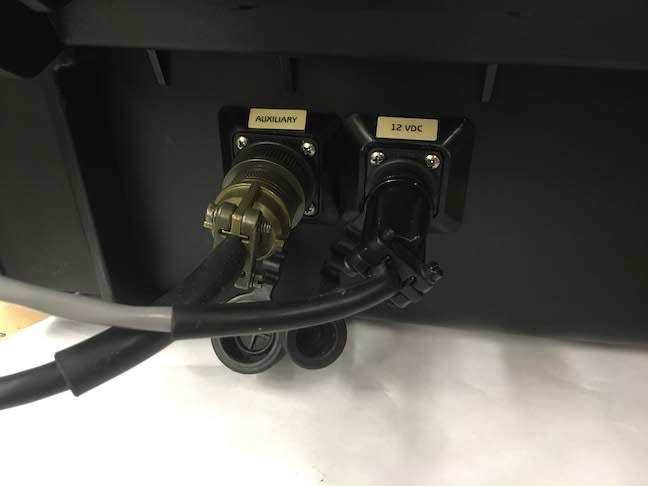
\includegraphics[width=0.8\linewidth]{pictures/ExternalPlugs} 

}

\caption{External plugs for the 2-pin and 6-pn cables}\label{fig:ExternalPlugs}
\end{figure}

\hypertarget{control-box-plugs}{%
\subsection{Control box plugs}\label{control-box-plugs}}

Inside the MUX, the control box (Figure \ref{fig:MUXLayout}) itself is connected via plugs to the 2-pin and 6-pin wires, and to the solenoid valves. The peristaltic pump is directly connected via its wires thanks to a screw terminal. Normally, there is no need to ever touch at any of these plugs. But should the user need it, it is possible to undo the control box from the rest, and or to change a solenoid valve and easily replace it if needed.

For illustration, the MUX power plugs, as well as the valve and the RS485 plugs on the control box. The 12V coming from the Con::nect Box are plugged in the control box as illustrated in Figure \ref{fig:ControlBoxConnection12V} below.

\begin{figure}

{\centering 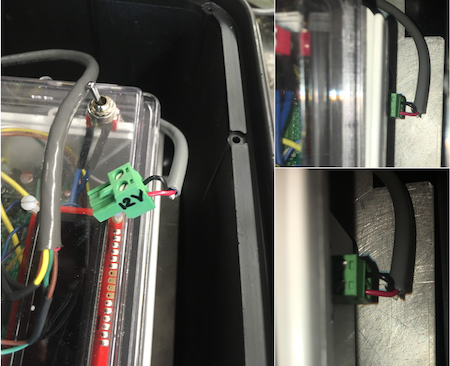
\includegraphics[width=0.8\linewidth]{pictures/ControlBoxConnection12V} 

}

\caption{12 V Connection between the control box and the external plug}\label{fig:ControlBoxConnection12V}
\end{figure}

The Signal input and the communication wires coming from the Con::nect Box are plugged in the control box as illustrated in Figure \ref{fig:ControlBoxConnectionValveRS485} below.

\begin{figure}

{\centering 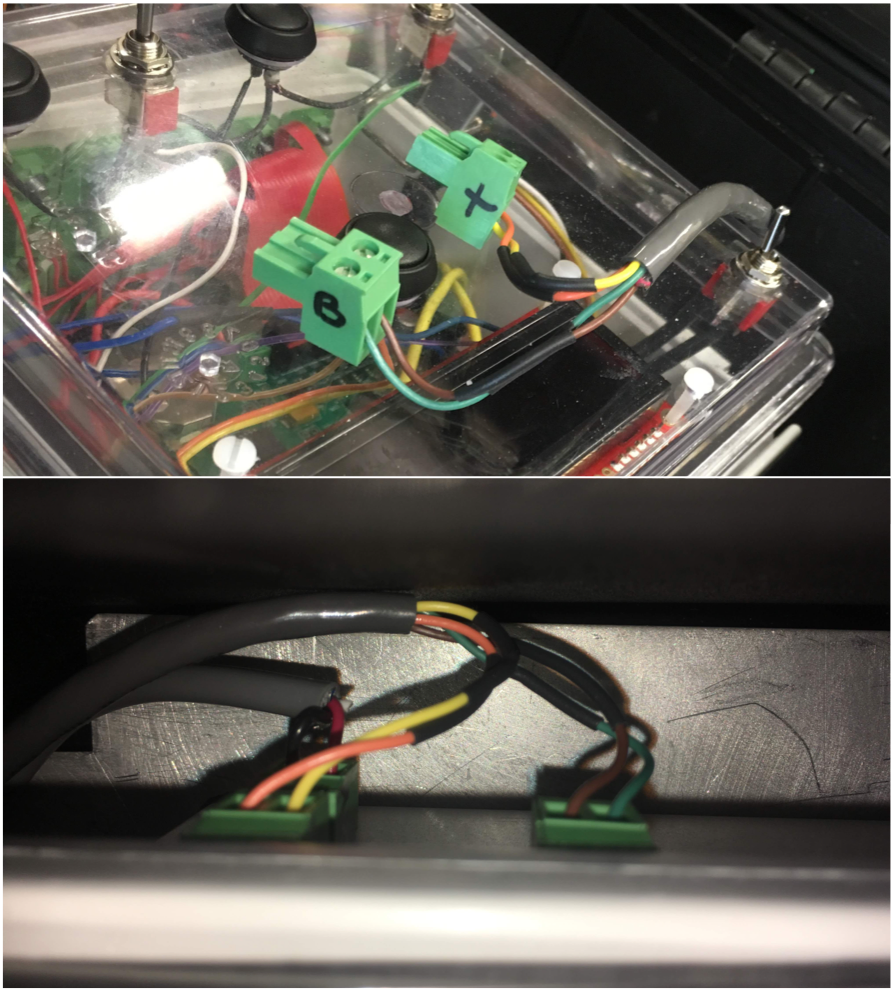
\includegraphics[width=0.8\linewidth]{pictures/ControlBoxConnectionValveRS485} 

}

\caption{12 V Connection between the control box and the external plug}\label{fig:ControlBoxConnectionValveRS485}
\end{figure}

\hypertarget{how-it-works}{%
\section{How it works}\label{how-it-works}}

peristaltic pump

change clock time

Manual pump

General functioning on/off

\hypertarget{how-to-start}{%
\section{How to start}\label{how-to-start}}

\hypertarget{sd-card}{%
\subsection{SD card}\label{sd-card}}

\hypertarget{config-file}{%
\subsection{Config file}\label{config-file}}

\hypertarget{rinsing-options}{%
\subsection{Rinsing options}\label{rinsing-options}}

\hypertarget{how-to-change-the-clock}{%
\section{How to change the clock}\label{how-to-change-the-clock}}

\hypertarget{how-to-pump-manually}{%
\section{How to pump manually}\label{how-to-pump-manually}}

\hypertarget{how-to-trigger-the-mux-manually}{%
\section{How to trigger the MUX manually}\label{how-to-trigger-the-mux-manually}}

\hypertarget{the-files-you-get}{%
\section{The files you get}\label{the-files-you-get}}

\hypertarget{trouble-shooting}{%
\section{Trouble shooting}\label{trouble-shooting}}

\hypertarget{the-mux-sensor-system}{%
\chapter{The MUX-sensor system}\label{the-mux-sensor-system}}

\hypertarget{the-general-design-principles-for-the-mux}{%
\section{The general design principles for the MUX}\label{the-general-design-principles-for-the-mux}}

An exert from our first paper \citep{Birgand2016-to} summarizes the philosophy behind the MUX:

\begin{quote}
To remain affordable, the system uses a single highfrequency automatic water quality probe as the central analytical
instrument to which water from different sampling sites (hereafter, point sources) are pumped via {[}the MUX{]}. Our design criteria when constructing the {[}MUX{]} system were: (1) to have the capacity of obtaining hourly or sub-hourly samples for measuring multiple point sources, (2) to be able to pump water from the point sources to the probe to overcome at least 3 m of head difference, (3) to be able to run on 12 volts (V) direct current (DC) power for field deployment, and (4) that the coupled {[}MUX{]}-water quality probe system functioned entirely automatically. An acceptable compromise for these criteria was to design {[}the MUX{]} that enabled sampling from up to 12 point source sites located within {[}30{]} m of the central probe. {[}\ldots{}{]}.
\end{quote}

\begin{quote}
As the in situ field spectrophotometer can only collect one measurement at a time on fixed time intervals, we designed and built {[}the MUX{]} to sequentially pump and purge water from each point source to the probe, in synchrony with the probe measurements, and cycle through the sequence of measurements to obtain at least hourly time resolution of data collection at each source. To maintain the water quality probe's capability of measuring small suspended particle concentrations, we chose 3.18 mm internal diameter flexible tubing as a sampling conduit of water from the point source to the probe, fitted with 1.5 mm mesh screens at the source {[}\ldots{}{]}. Consequently, the coupled {[}MUX{]}-water quality probe system is well suited for applications where the source sampling volume is not limited and does not affect the process or system studied.
\end{quote}

\hypertarget{the-different-parts-of-the-mux-sensor-system}{%
\section{The different parts of the MUX-sensor system}\label{the-different-parts-of-the-mux-sensor-system}}

\hypertarget{bidirectional-flow-and-rinsing-purposes}{%
\subsection{Bidirectional flow and rinsing purposes}\label{bidirectional-flow-and-rinsing-purposes}}

In continuous flow laboratory analytical equipment, the flow in the tubing is unidirectional, and the measuring cuvette is rinsed by the carrier solution and color reagent between samples to essentially eliminate cross-contamination between samples. In our case, although we are using the Spectro::lyser as an \emph{in situ} laboratory instrument, there is no carrier fluid for rinsing between samples. To minimize cross contamination between samples, the idea we developed was to reverse flow and purge the instrument cuvette from its water instead. This is the reason for using a peristaltic pump. Now water can be purged either to the sampling port or to a port dedicated to waste.

This addresses the cross contamination, but not the fouling that may occur as is often the case on the instrument optics. For this reason, the MUX has an embedded rinsing procedure where it is possible to use acid or other solutions for rinsing. The overall general MUX-sensor setup is summarized in Figure \ref{fig:WorkLayout} below.

\begin{figure}

{\centering 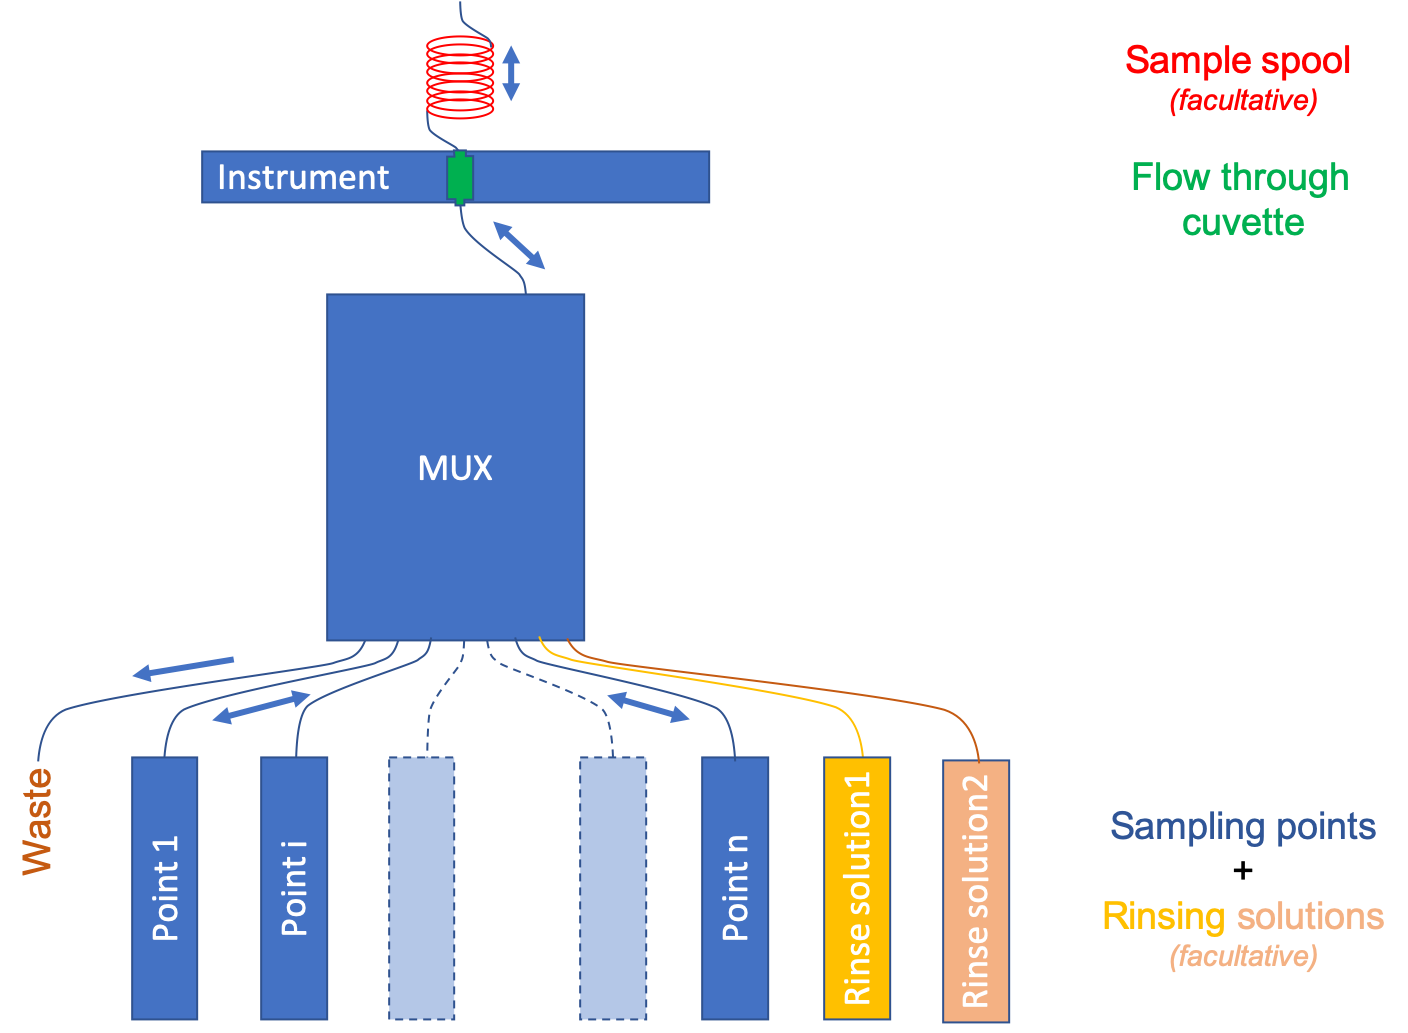
\includegraphics[width=0.8\linewidth]{pictures/WorkLayout} 

}

\caption{The MUX in relationship with the sampling points, rinsing solutions, the instrument and its flow-through cuvette, and a sample loop}\label{fig:WorkLayout}
\end{figure}

In Figure \ref{fig:WorkLayout} above, \emph{n} sampling ports are activated, while two of the ports are dedicated to a \emph{rinsing solution 1} and a \emph{rinsing solution 2}. The MUX has 12 sampling ports and a 13\textsuperscript{th} port for waste if desired. The number or rinsing solutions used, therefore reduces the number of available ports for measured points. In the case of Figure \ref{fig:WorkLayout} above, a maximum of 12 - 2 = 10 ports remain available for point sampling.

Sampled water from any sampling point, including the rinsing solutions, can be purged to any port, including the dedicated waste port (port 13 in the MUX box), or the same port used for sampling, or any other port of the user's choice.

At the instrument, water is pumped through a flow-through cuvette. This allows to pump water beyond the cuvette and allow for rinsing of the whole manifold and of the cuvette with the new sample. We have found that a good practice to minimize cross contamination is to pump water at least 4 times beyond the volume of the cuvette. For use with the Spectro::lyser with a 35 mm opening, we recommend to use the cuvette 1-Q-10/SBTX2-8/10X20 from Starnacell\textsuperscript{®}. It has a 10 mm path length, is made of quartz, which lets the UV light through, and has a large collar, which make cleaning much easier.

Eventually during a measurement campaign, it is necessary to compare the instrument measured concentrations to those of the laboratory. For this, it is sometimes a good idea to add a \emph{sampling spool} made of tubing curled together. We recommend that the spool allows for large enough a volume corresponding to the one needed for lab analyses, but small enough such that the initial water that has served to rinse the MUX and the cuvette be beyond the spool such that when purging only `clean water' be used for lab sampling.

\hypertarget{basic-sequence-of-events}{%
\subsection{Basic sequence of events}\label{basic-sequence-of-events}}

In the MUX \emph{config.txt} file (see further details later), the user specifies the desired sampling interval. During initialization, the MUX puts the Spectro::lyser in \emph{logger mode}, which means that the instrument will, with no live connection to a computer, automatically take measurements at the indicated time interval.

The Spectro::lyser sequence of actions (Figure \ref{fig:BasicSequence}) is thus to first send a 12V signal measurable at the `valve' output in the Con::nect box. Again, this is the way the Spectro::lyser deals with fouling. After a given time, referred to as \emph{clean wait} in the \emph{config.txt} file and in Figure \ref{fig:WorkLayout}, the instrument takes a measurement. A measurement consists in two series of light bursts accompanied by a series of beeps. There are about 9 seconds between the first and the last beep. After that, it takes the Spectro::lyser about 25 seconds to analyze its measurement and make available its absorbance fingerprint and its calculated concentrations (Figure \ref{fig:BasicSequence}).

\begin{figure}

{\centering 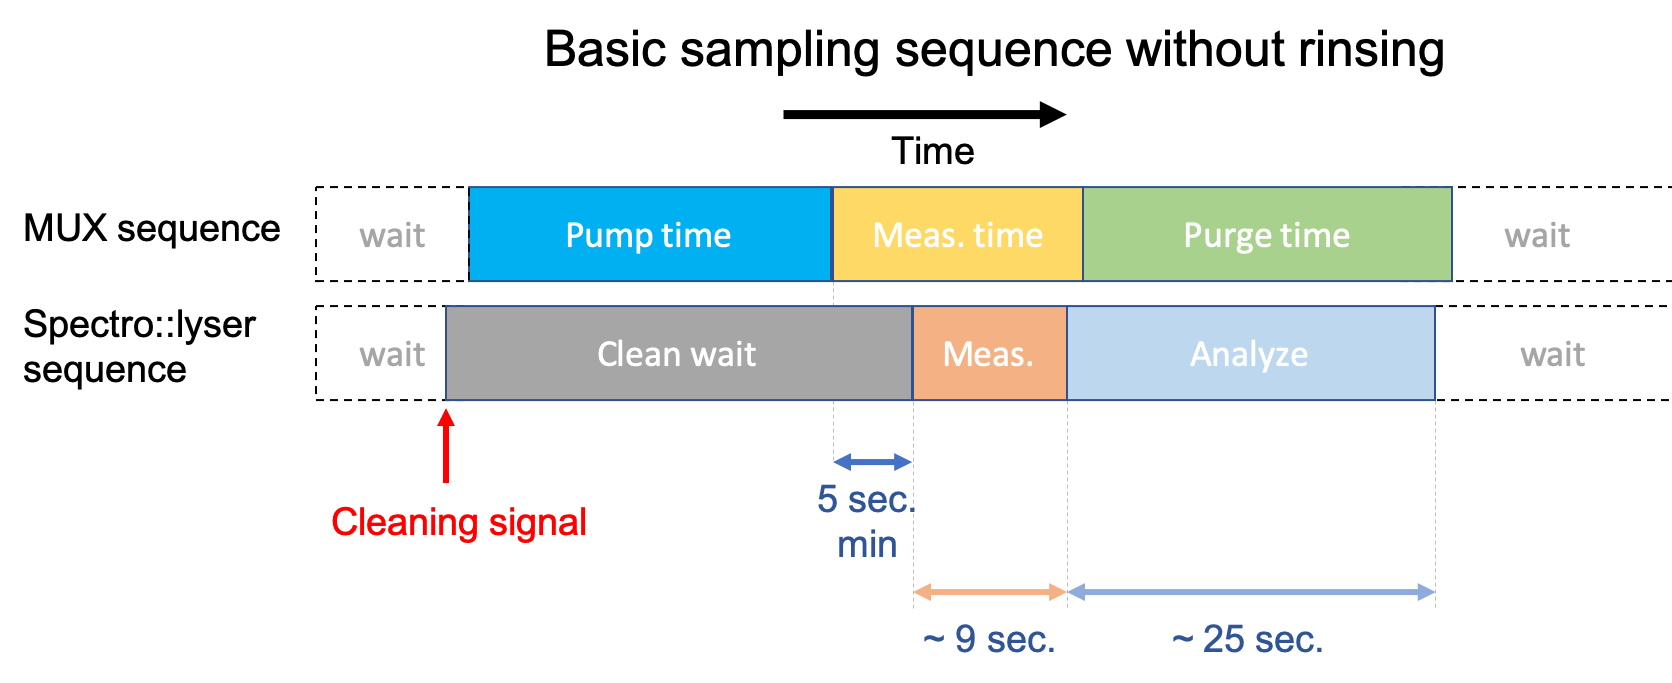
\includegraphics[width=0.8\linewidth]{pictures/BasicSequence} 

}

\caption{The MUX in relationship with the sampling points, rinsing solutions, the instrument and its flow-through cuvette, and a sample loop}\label{fig:BasicSequence}
\end{figure}

The idea with the MUX is to have water to be analyzed in the measuring chamber or cuvette when the Spectro::lyser does its measurement. Once the MUX `hears' the \emph{cleaning signal} from the Spectro::lyser (Figure \ref{fig:BasicSequence}), it starts its pumping for a \emph{pump time} defined in the \emph{config.txt} file. The \emph{pump time} corresponds to the time it takes for water to go from its sampling point to the instrument cuvette, to which one must add the number of seconds necessary to rinse the equivalent of at least 4-5 times the cuvette volume. For some applications, there is no limit on the available volume of water to be analyzed. In these cases, one might want to add 5-6 seconds more on the \emph{pump time}. For other applications, the available volume might be limited, and it might be necessary to limit the pump time to the strict minimum prescribed here.

The \emph{pump time} and the \emph{clean wait} times are thus intrinsically linked. The \emph{clean wait} time has to be equal to the pump time plus at least 5 seconds to let water in the cuvette `rest' and let all micro air bubbles to stop moving to obtain a reliable and consistent reading by the Spectro::lyser. Keep in mind that there are about 1-2 seconds delay between the \emph{cleaning signal} and the time when the pumping starts (Figure \ref{fig:BasicSequence}).

There are two important things to realize here:

\begin{enumerate}
\def\labelenumi{\arabic{enumi}.}
\item
  In reality, the \emph{pump time} may vary from sampling point to the next as it is preferable to pump the least amount of time per port to save energy and pump tubing. The \emph{pump time} for each port is defined in the \emph{config.txt} file. However, the \emph{clean wait} time corresponds to a parameter from the Spectro::lyser, and the same value applies to all sampling points. As a result, the \emph{clean wait} time \textbf{must correspond to the longest \emph{pump time} + 5 seconds} (Figure \ref{fig:TimingsSeveralPorts}).
\item
  Because it always takes the same amount of time between the \emph{cleaning signal} and the last beep of the Spectro::lyser measurement, and, because the \emph{pump time} may vary from one sampling point to the next, the (on the MUX side) \textbf{sum of \emph{pump time} + the MUX \emph{measurement time}} should also be the same and be equal to (on the Spectro::lyser side) \textbf{the \emph{clean wait} time + the 9 sec.~of measurement time + at least 2 seconds past the last measurement} (Figure \ref{fig:TimingsSeveralPorts}).
\end{enumerate}

As a result, the \emph{measurement time} from the MUX must be adjusted (in the \emph{config.txt} file) accordingly as illustrated in Figure \ref{fig:TimingsSeveralPorts}

\begin{figure}

{\centering 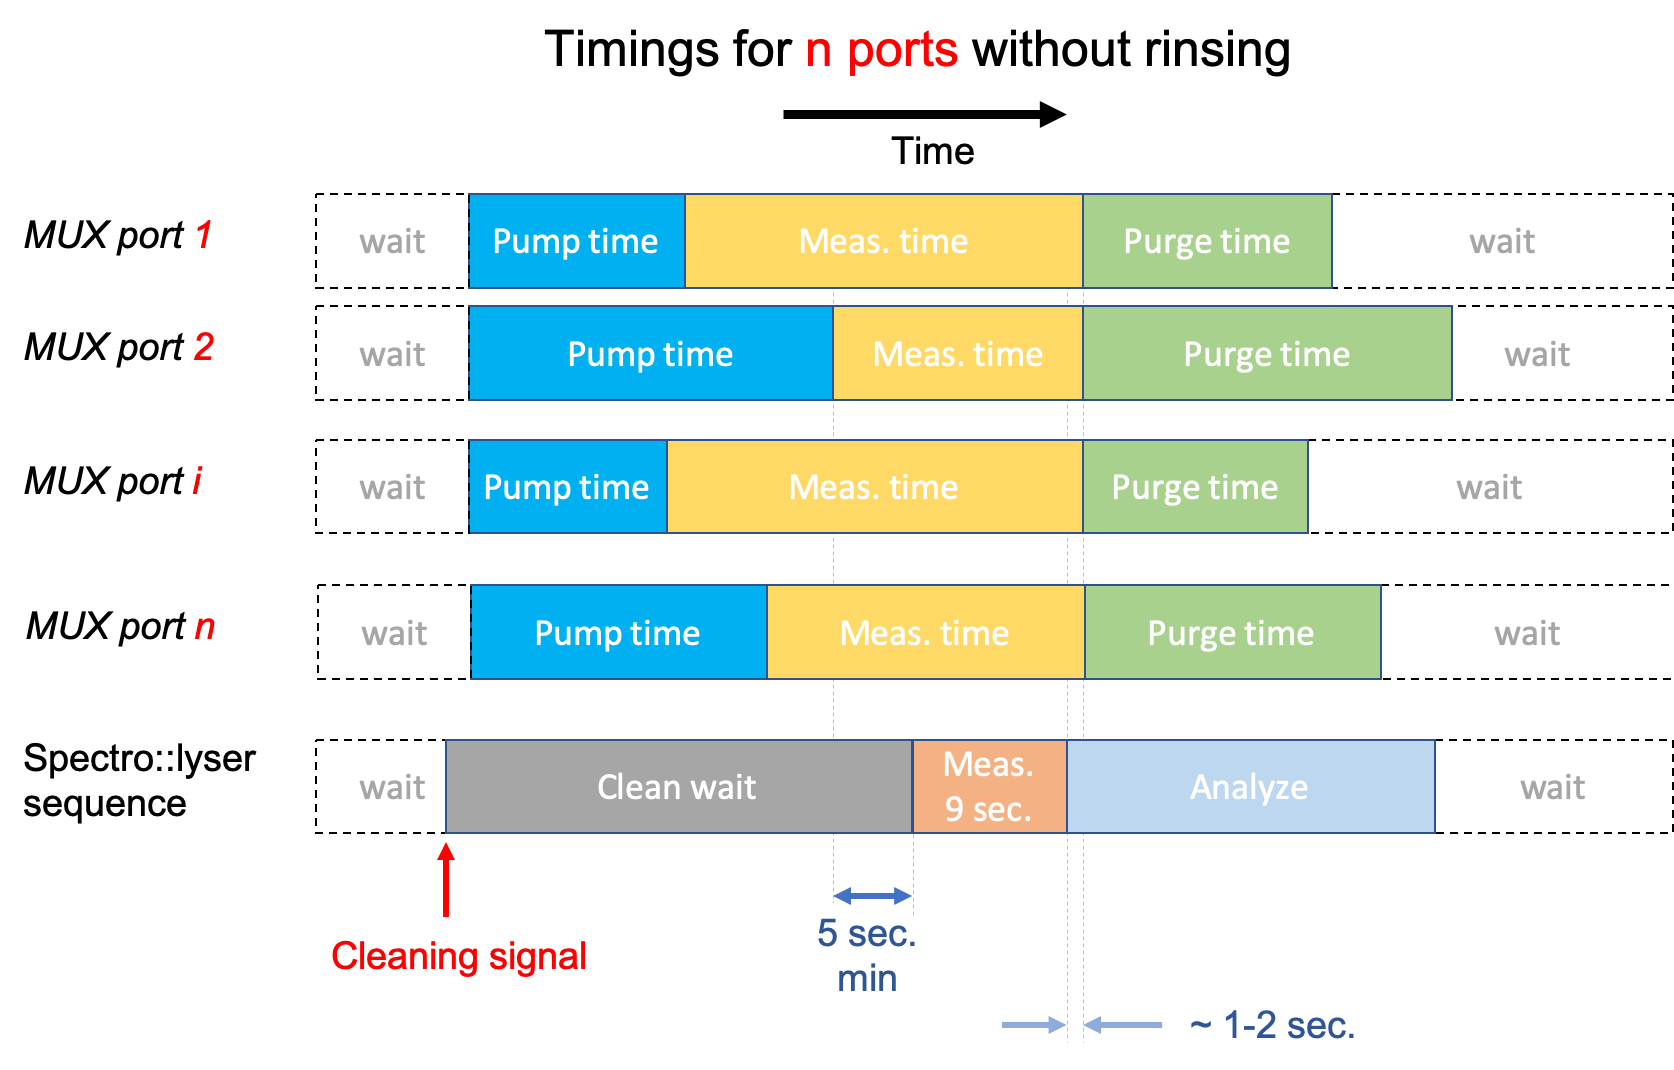
\includegraphics[width=0.8\linewidth]{pictures/TimingsSeveralPorts} 

}

\caption{The MUX in relationship with the sampling points, rinsing solutions, the instrument and its flow-through cuvette, and a sample loop}\label{fig:TimingsSeveralPorts}
\end{figure}

\bibliography{book.bib,packages.bib}


\end{document}
